\chapter{Opis projektnog zadatka}
		
		\textbf{\textit{Uvod}}\\
		
		\textit{Cilj projekta "Medicinska rehabilitacija" je razvoj programske podrške za stvaranje istoimene web aplikacije koja će omogućiti korisnicima jednostavno naručivanje za fizikalnu terapiju i medicinsku rehabilitaciju. Korisnici u našem slučaju su bolesnici koji su se ozlijedili te trebaju stručnu pomoć. Zadatak nam je omogućiti intuitivno korisničko sučelje kako bi olakšali korištenje aplikacije bolesnicima, ali i zdravstvenim djelatnicima.}
		
		\textit{Glavna motivacija bila nam je modernizacija hrvatskog zdravstva. Vjerujemo kako pacijentima nije drago zvati mobitelom svoje doktore znajući da su pretrpani poslom, a također im je dosta čekanje na odgovor zdravstvenog djelatnika kada im se pošalje mail. S druge strane nije ni zdravstvenim djelatnicima lako odgovarati na sve te silne poruke. Ovom aplikacijom bismo omogućili pacijentima da biraju dostupan termin koji njima najbolje odgovara, a doktore poštedili dodatnog posla.}
		
		\textit{Između ostalog ova bi aplikacija omogućivala liječnicima praćenje poboljšanja zdravstvenog stanja pacijenata. Ako se pacijenti prvi puta naručuju za terapiju potrebna je registracija, a svaki sljedeći put je nužna prijava u sustav. Za registraciju potrebni su sljedeći podaci: }
		\begin{packed_item}
			\item \textit{ime i prezime}
			\item \textit{korisničko ime}
			\item \textit{lozinka}
			\item \textit{e-mail adresa}
			\item \textit{OIB}
			\item \textit{spol}
			\item \textit{datum rođenja}
		\end{packed_item}
		
		\textit{Administrator gornje podatke mora verificirati iz središnjeg informacijskog sustava zdravstvene zaštite. Bolesnici prilikom prijave moraju navesti vrstu i opis svojih oboljenja, zahtijevani postupak liječenja te liječnika koji ih je uputio na rehabilitaciju. Nakon toga moraju odabrati neki od dostupnih termina. Ako se ne radi o prvom dolasku u ustanovu zahtijeva se i prikaz reference na već obavljeni postupak u toj ustanovi. Zdravstveni djelatnici dodjeljuju termine tako da vode brigu o ukupnom kapacitetu opreme/uređaja, kapacitetu prostorija, broju dostupnih djelatnika te trajanju svakog zahvata. Nakon dobivenog termina bolesniku dolazi e-pošta sa terminom te ostalim dodatnim informacijama. U slučaju neočekivanih promjena djelatnik može kontaktirati bolesnika putem e-pošte. Radno vrijeme ustanove u kojoj se provodi rehabilitacija je svakim radnim danom od 8 do 20 sati. Ustanova ima pravo odrediti određene slobodne dane na temelju blagdana ili praznika.}\\
		
		\textbf{\textit{Primjer sličnog rješenja}}\\
		
		\textit{Primjer sličnog rješenja je aplikacija "Buker". To je aplikacija koja omogućuje naručivanje za termin u određenim salonima (npr. frizerskim ili kozmetičkim). }
		
		\textit{Registracija je omogućena putem telefonskog broja gdje korisnik mora verificirati svoje podatke ili još jednostavnije putem google računa. Za registraciju u ovaj sustav potrebno je ispuniti svoje ime, prezime te e-mail adresu. Naravno ovdje se neće tražiti puno informacija kao u našem sustavu niti se očekuje toliko stroga kontrola istinitosti podataka. }
		
		\begin{figure}[H]
			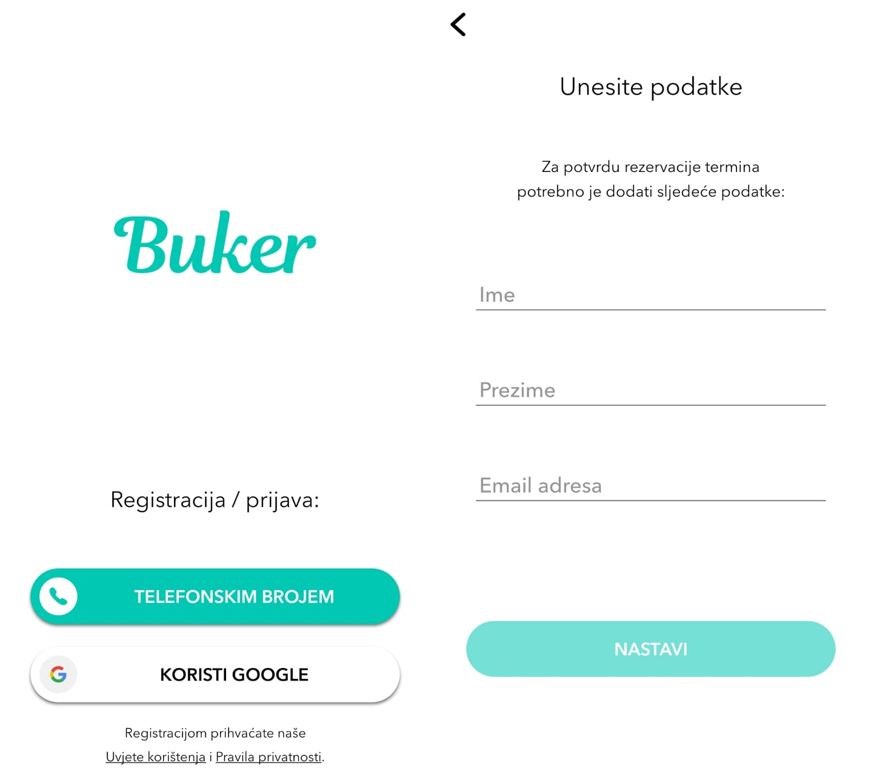
\includegraphics[scale=0.6]{slike/Buker-registracija.PNG} %veličina slike u odnosu na originalnu datoteku i pozicija slike
			\centering
			\caption{Registracija u sustav "Buker"}
			\label{fig:promjene}
		\end{figure}
		
		\textit{Zatim imamo mogućnost odabrati kategoriju te u pojedinoj kategoriji određeni salon gdje dobijemo prikaz njihovih usluga. Označimo onu uslugu koju želimo te kliknemo na dugme "Termini".}
		
		\begin{figure}[H]
			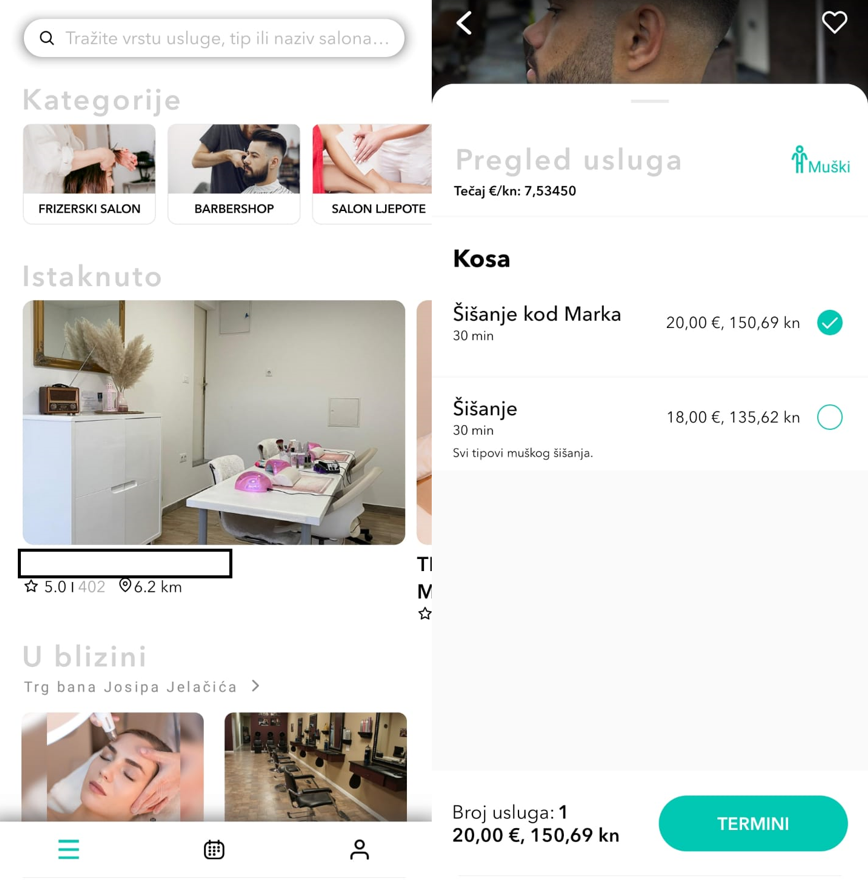
\includegraphics[scale=0.6]{slike/Buker-odabir.PNG} %veličina slike u odnosu na originalnu datoteku i pozicija slike
			\centering
			\caption{Odabir kategorije i usluge}
			\label{fig:promjene}
		\end{figure}
		
		\textit{Na kraju nam preostaje odabir dostupnih termina. Naravno ovdje slobodni termini ovise isključivo o radnom vremenu salona, zauzeću od nekog drugog klijenta te trajanju samog zahvata. Kod naše aplikacije termini ovise dodatno o kapacitetu opreme/uređaja, kapacitetu prostorija i broju dostupnih djelatnika.}
		
		\begin{figure}[H]
			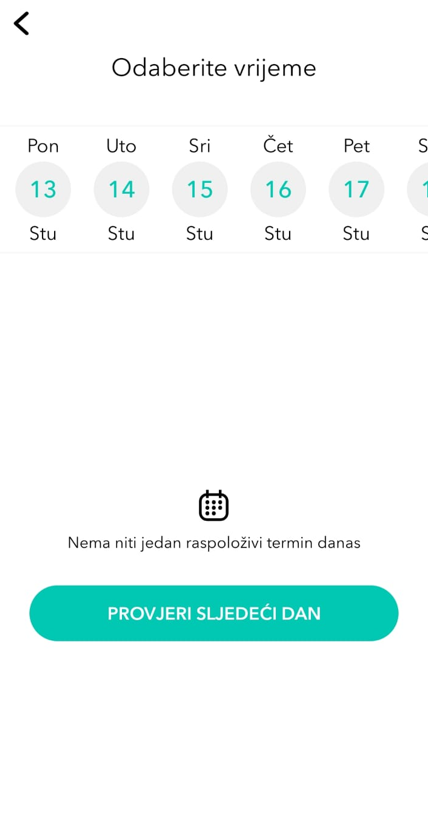
\includegraphics[scale=0.6]{slike/Buker-odabir-termina.PNG} %veličina slike u odnosu na originalnu datoteku i pozicija slike
			\centering
			\caption{Odabir termina}
			\label{fig:promjene}
		\end{figure}
		
		\textbf{\textit{Dodatno pojašnjenje}}\\
		
		\textit{Korisnici sustava su:}
		
		\begin{packed_item}
			\item \textit{pacijenti}
			\item \textit{zdravstveni djelatnici}
			\item \textit{administrator}
		\end{packed_item}
		
		\textit{Svaki od te tri skupine korisnika ima različita dopuštenja. Djelatnici ustanove mogu vidjeti sve bolesnike i tretmane koji su im dodijeljeni. Nakon svakog obavljenog postupka djelatnik u sustav registrira pacijenta, a nakon završenog ciklusa zapisuje postignute rezultate. Pacijenti mogu vidjeti samo svoje tretmane. Administrator upravlja čitavim sustavom. Njemu su dostupni svi podaci i može definirati sve što je potrebno za ispravan rad sustava.}
		
		\textit{Za unesene podatke prilikom registracije u aplikaciju osigurat ćemo provjeru konzistentnosti s podacima iz baze podataka. Nakon toga korisnik postaje pacijent, izabire datum te ima mogućnost otkazati termin 1 dan prije početka tog termina.}
		
		\textit{Opreme, odnosno uređaji koje posjeduje ustanova se kategoriziraju. Spomenuli smo da slobodni termini ovise o ukupnom kapacitetu opreme/uređaja. Naravno da nije isto ako je čovjeku oštećena ruka ili noga. Tu se radi o drugoj opremi koju će zdravstveni djelatnik morati upotrijebiti za liječenja pacijenta. Dakle, korisnik kojemu je ozljeđena ruka neće zauzimati opremu korisniku kojemu je ozljeđena noga. Očekujemo da će broj oprema/uređaja za određeni dio tijela ipak biti veći od jedan, no svakako će biti ograničen.}
		
		\textit{Korisnik se u sustav prijavljuje upisivanjem korisničkog imena te svoje lozinke koja mora zadovoljavati određena pravila. Lozinka mora imati minimalno 8 znakova, od čega mora biti minimalno jedno veliko slovo te jedna znamenka. Ako korisnik prilikom registracije i smišljanja lozinke nije zadovoljio navedena pravila, dobit će upozorenje što mu nedostaje za ispravnu lozinku.}\\
		
		\textit{Aplikacija će imati \textbf{n} stranica. Te stranice su redom: Naslovna stranica, stranica za registraciju, stranica za prijavu, \textbf{stranica za promjenu lozinke}, stranica za odabir termina, stranica za administratora gdje administrator održava sustav i potvrđuje registracije, stranica gdje djelatnik potvrđuje termine, \textbf{"help page" koja objašnjava funkcionalnost aplikacije} i stranica u kojoj se provjerava status pacijenta (odnosno njihovu povijest sa tom ustanovom)}.\\
		
		\textbf{\textit{Opseg projekta}}\\
		
		\textit{Na projektu radi 7 osoba, studenata FER-a. Projekt se radi u edukativne svrhe provjere znanja studenata u sklopu predmeta "Programsko inženjerstvo". Vremensko ograničenje za prvu verziju projekta je 7 tjedana, a druga verzija (odnosno cijeli projekt) mora biti isporučen u roku od 14 tjedana od početka rada. Ukupan broj potrošenog vremena otići će najviše na sami rad oko projekta, ali značajan dio vremena otići će i na sastanke uživo gdje će tim redovito raspraviti o tjednom napretku.}
		
		\eject
		